After the UTC-day quota reset restored API access, we evaluated all fixed outputs with the originally planned Claude Haiku 4.5 rubric. This late audit followed inspection of the local results; it did not change any direction, strength, prompt, or generated answer. It contributes 1,570 additional evaluations: 1,260 intervention answers, 250 natural audit excerpts, and 60 quality corruptions. Complete raw responses are retained, including explanatory text when the service returned more than the requested JSON.

Unlike Mistral, Claude's AI-style ratings distinguish known provenance on both audits: HC3 AUROC 0.856 [0.804, 0.903] and HAP-E 0.849 [0.788, 0.906]. Its $+1$ minus $-1$ authorship-style contrast is 5.67 [2.90, 8.93] points. This supplies a second kind of evidence that the HC3 direction affects AI-like wording, beyond classifier scores. It remains an LLM judgment rather than a human perceptual experiment.

The nuisance comparison is less favorable to a distinct style axis. The formality control has a style contrast of 8.83 [5.58, 12.43], and the authorship contrast does not exceed it (difference $-3.17$ [$-7.57$, 1.23]). Orthogonalization reduces the style contrast to 1.40 [0.00, 3.20], a reduction of 4.27 [1.90, 6.98] relative to the original direction. In contrast, its trained-detector effects remain substantial. Thus detector movement after nuisance removal is stronger evidence for detection-related features than for a distinct AI-style control. The HAP-E direction has a smaller positive Claude style contrast of 2.50 [1.33, 3.67], agreeing with Desklib rather than the reversed RoBERTa response.

\begin{figure*}[t]
\centering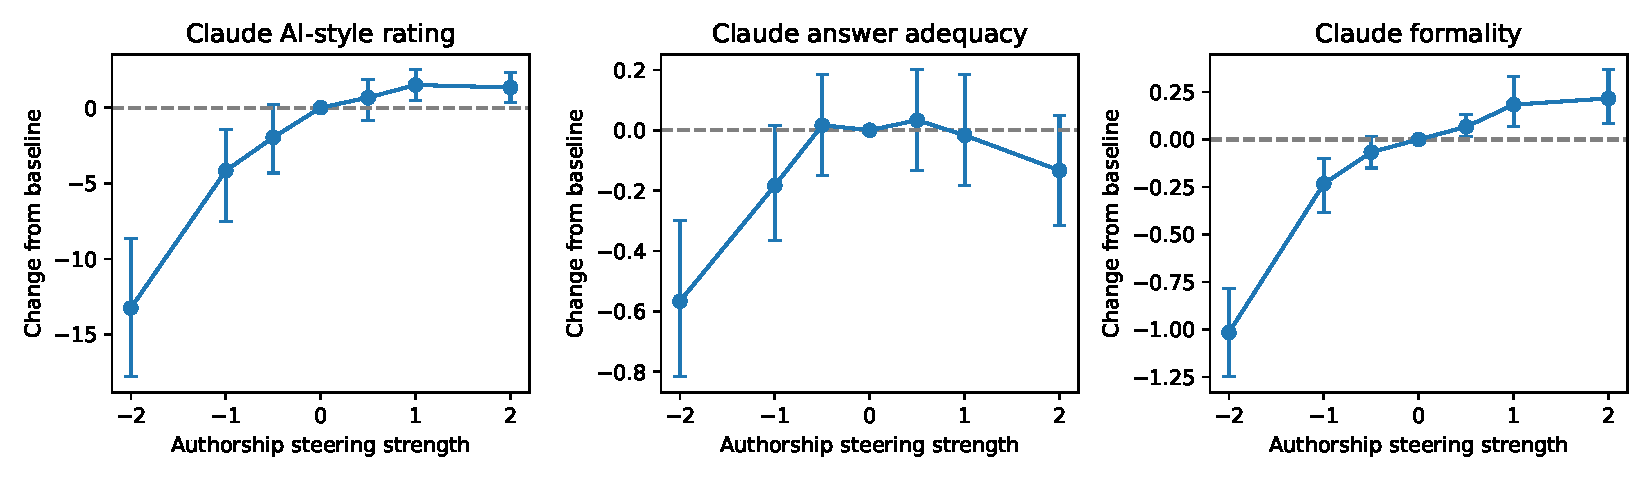
\includegraphics[width=\textwidth]{figures/claude_dose.pdf}
\caption{Late blinded Claude audit of unchanged generations. Negative authorship steering reduces rated AI-like style, but the strongest intervention also reduces answer adequacy and formality. These results were obtained after the initial local study, using its original rubric.}
\label{fig:claude}
\end{figure*}

Most importantly, Claude is substantially stricter about quality. Baseline mean adequacy is 3.10, versus Mistral's 4.78; only 23 of 60 baseline answers pass the joint threshold, versus all 60 under Mistral. At $-2$, AI style falls by 13.25 [$-17.80$, $-8.63$] points, but adequacy falls by 0.567 [$-0.817$, $-0.300$] and coherence by 0.750. At $-1$, AI style falls by 4.17 [$-7.50$, $-1.47$], with adequacy change $-0.183$ [$-0.367$, 0.017]. Only 16 baseline/$-1$ pairs satisfy Claude's quality threshold; their style change is $-1.69$ [$-7.56$, 1.88]. This small, selected subset cannot establish quality-preserving humanization.

Claude also detects known corruption: on the 20-answer quality audit, shuffling reduces coherence from 4.45 to 1.15, and unrelated answers reduce adequacy from 3.20 to 1.00. Agreement on gross corruption therefore does not imply agreement on the adequacy of plausible natural answers. The late audit materially weakens claims based on the original quality filter. All Claude condition means, changes, and quality-qualified effects are reported in Table~\ref{tab:claudeall}.
